\chapter{The models}
\label{chapter3}

\section{Nowcasting: the dynamic factor model}
\label{chapter3_section1}

The dynamic factor model is the econometric methodology used by Now-casting.com to produce its predictions. The model has been originally proposed in \cite{Giannone2005}, but the main reference is the contribution of \cite{Giannone2008}, which essentially repeats the same methodology and provides a detailed technical appendix. \cite{Doz2011} provides deeper theoretical developments, justifying the statistical correctness of the two-steps methodology developed below. \cite{Banbura2010} proposes the same methodology with an alternative use of the EM algorithm in place of the Kalman filter.

The dynamic factor model is a mixed frequency model for nowcasting. More specifically, it aims at predicting quarterly GDP growth from many higher-frequency, monthly economic variables. The dataset used by \cite{Giannone2008} is consistent with the one proposed for this project, except that it is larger (around 250 features, most variables being decomposed into sub-components). Because a large number of data series in the model would lead to the curse of dimensionality issue, the authors propose to reduce the many series to a few dynamic factors that are in turn be used to predict real GDP.


\subsection{Formulation}
\label{chapter3_section1_subsection1}

Assume that are $n$ monthly variables involved in the model over $T$ periods. Denote by $x_{i,t}$ the value of variable $i$ at period $t$, with $i = 1, \cdots, n$ and $t = 1, \cdots, T$. It is assumed that each variables is linearly related to a small number $r$ of factors with $r \ll n$. Denoting by $f_{j,t}$ the value of factor $j$ at period $t$, the relation obtains as:

\begin{equation}
x_{i,t} = \mu_i + \lambda_{i1} f_{1,t} + \cdots +  \lambda_{ir} f_{r,t} + \xi_{i,t} \hspace{2cm}
\xi_{i,t} \sim \No(0, \psi_i)
\label{equation_c1_s1_ss1_1}
\end{equation}

Stacking then all the $n$ variables in a single vector $x_t$, the equation rewrites compactly as:

\begin{equation}
x_t = \mu + \Lambda f_t + \xi_t \hspace{2cm} \xi_t \sim N(0, diag(\psi))
\label{equation_c1_s1_ss1_2}
\end{equation}	

where $x_t$, $\mu$, $f_t$, $\xi_t$ and $\psi$ are $n$-dimentional vectors, and $\Lambda$ is a $n \times r$ matrix of factor loadings. It is further assumed that the dynamic factors follow an auto-regressive process:

\begin{equation}
f_t = A f_{t-1} + B u_t \hspace{2cm} u_t \sim \No(0, I_q)
\label{equation_c1_s1_ss1_3}
\end{equation}

where $A$ is a $r \times r$ matrix of autoregressive coefficients, and $u_t$ is a $q$-dimensional vector of common shocks assume to drive the dynamics of the factors. Typically, we set $q \leq r$ in order to capture the lead and lag relations among variables.

Finally, denote by $\hat{y}_t$ the nowcast for real GDP growth at time $t$. It is related to the value of the dynamic factor by the following equation:

\begin{equation}
\hat{y}_t = \alpha + \beta \hat{f_t}
\label{equation_c1_s1_ss1_4}
\end{equation}

where $\hat{f_t} = \Ex(f_t|\Omega_t)$, that is, $\hat{f_t}$ is the optimal projection of $f_t$, given the available information set $\Omega_t$.


\subsection{Estimation}
\label{chapter3_section1_subsection2}

If the series of dynamic factors $f_t$ was known, estimating the model would be straightforward. However, they cannot be estimated directly from \ref{equation_c1_s1_ss1_2} since the parameters $\mu$ and $\Lambda$ are also unknown. For this reason, \cite{Giannone2008} propose a procedure in 2 steps: first, estimate a preliminary version of the $r$ factors by applying PCA (principal component analysis) on $x_t$; second, estimate the model parameters from these raw factors, then use these parameters to obtain optimal projections of the factors from Kalman filtering. It is then trivial to obtain the predictions for GDP and the other features.

In details, the authors propose the following procedure:

\textbf{Algorithm 1: dynamic factor model} \vspace{3mm} \\
1. Feature standardization: \\
Standardize the data so that it has zero mean and unit variance: $z_{i,t} = (x_{i,t} - \hat{\mu}_i) / \hat{\sigma}_i$. Then calculate the correlation matrix $S = \frac{1}{T} \sum_{t=1}^{T} z_t z_t'$. \\

\newpage

2. Principal component analysis:\\
denote by $D$ the $r \times r$ diagonal matrix with the $r$ largest eigenvalues of $S$ and by $V$ the corresponding $n \times r$ matrix of eigenvectors. A raw estimate of the dynamic factors obtains as: $f_t = V' z_t$.

3. Parameters for the feature dynamics: \\
$\Lambda = \sum_{t=1}^{T} z_t f_t' \left( \sum_{t=1}^{T} f_t f_t' \right)^{-1} = V$ \hspace{2cm}
$\psi = diag(S - VDV)$

4. Parameters for the factor dynamics: \\
$A = \sum_{t=2}^{T} f_t f_{t-1}' \left( \sum_{t=2}^{T} f_{t-1} f_{t-1}' \right)^{-1}$ \hspace{2cm}
$B = M P^{1/2}$ \\
where $P$ is the $q \times q$ diagonal matrix with the $q$ largest eigenvalues of $\Sigma$, M is the $r \times q$ matrix of corresponding eigenvectors, and $\Sigma$ is defined as: \\
$\Sigma = \frac{1}{T-1} \sum_{t=2}^{T} f_t f_t' - A \left( \sum_{t=2}^{T} f_{t-1} f_{t-1}' \right) A'$

5. Optimal projections of the factors: \\
Given that \ref{equation_c1_s1_ss1_2} and \ref{equation_c1_s1_ss1_3} are formulated in state-space form, they can be used to obtain optimal projections $\hat{f_t}$ of the factors from the Kalman smoother. Please refer to Appendix \ref{appendix3} for details on the Kalman filter procedure.

6. Parameters for GDP nowcasting: \\
With the projected factors $\hat{f_t}$ at hands, estimate \ref{equation_c1_s1_ss1_4} by OLS.


\subsection{Prediction}
\label{chapter3_section1_subsection3}

Once the model is trained, it is straightforward to obtain predictions. From \ref{equation_c1_s1_ss1_2}, predictions for the features at horizon $t+h$ can be obtained as:

\begin{equation}
\hat{x}_{t+h} = \mu + \Lambda \hat{f}_{t+h}
\label{equation_c1_s1_ss3_1}
\end{equation}

as for predictions for quarterly GDP, they obtain directly from \ref{equation_c1_s1_ss1_4} as:

\begin{equation}
\hat{y}_{t+h} = \alpha + \beta \hat{f}_{t+h}
\label{equation_c1_s1_ss3_2}
\end{equation}

Both predictions require $\hat{f}_{t+h}$. But $\hat{f}_{t+h}$ can be trivially obtained from the Kalman filter, by continuing the Kalman iterations up to period $t+h$.


\subsection{Application}
\label{chapter3_section1_subsection4}


The dynamic factor model is applied to the project dataset. Figure \ref{fig_c3_s1_ss2_1} provides an overview of the structural factors, both raw and smoothed by the Kalman filter, while Figure \ref{fig_c3_s1_ss2_2} plots actual GDP growth and the in-sample predictions obtained from the model.

\begin{figure}[H]
\centering
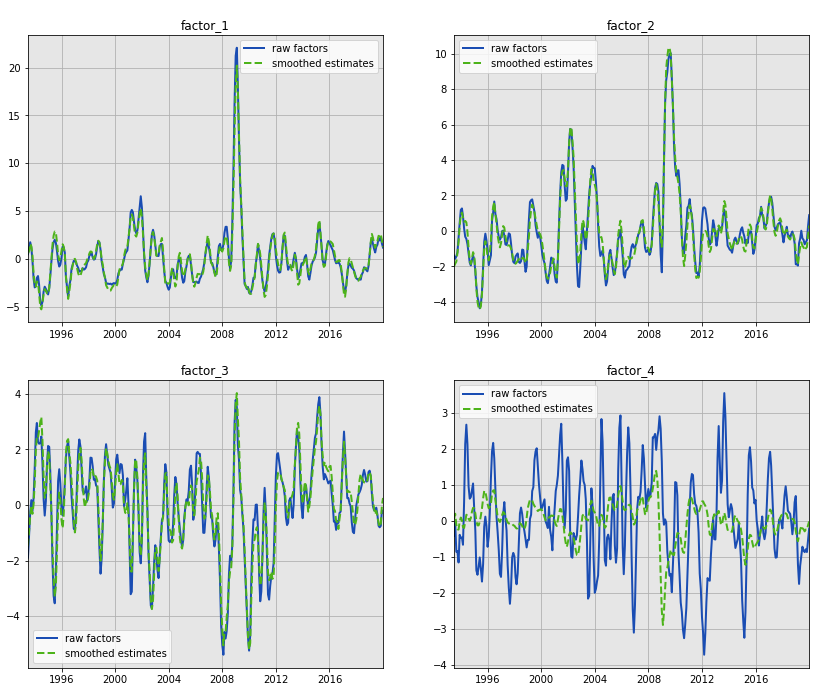
\includegraphics[scale=0.5]{images/structural_factors.png}
\caption{Structural factors for the project dataset}
\label{fig_c3_s1_ss2_1}
\end{figure}

\begin{figure}[H]
\centering
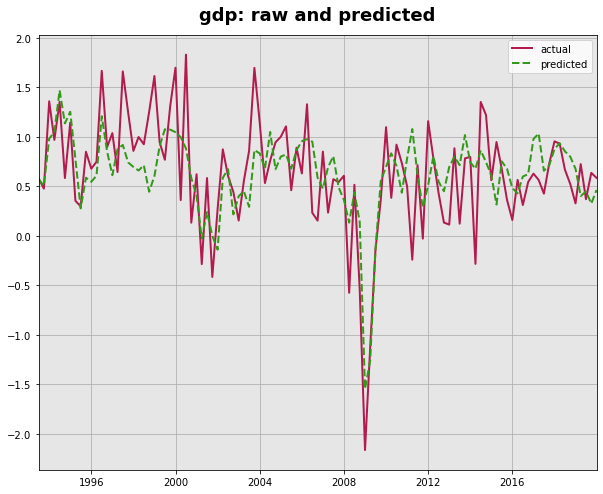
\includegraphics[scale=0.4]{images/dfm_gdp.png}
\caption{In-sample GDP: actual and predicted}
\label{fig_c3_s1_ss2_2}
\end{figure}

The discrepancy between the raw factors and their smoothed versions seems small, except for the final one for which the prediction differs considerably from the raw estimate. There seems to exist a significant correlation between GDP and the structural factors, though this correlation is negative for some factors. It is then informative to check which features contribute to the design of each factor, and hence have most explanatory power on GDP in the dynamic factor model. This information is reported in Figure \ref{fig_c3_s1_ss2_3}.

\begin{figure}[H]
\centering
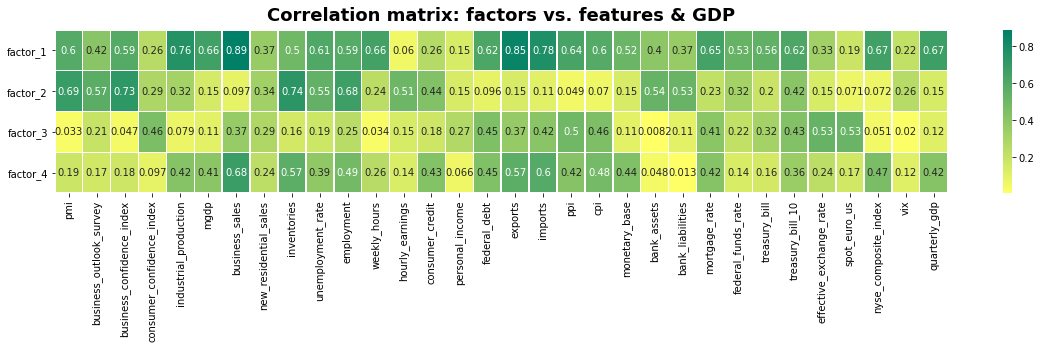
\includegraphics[scale=0.43]{images/factor_correlations.png}
\caption{Correlations: factors, features and GDP}
\label{fig_c3_s1_ss2_3} \vspace{-8mm}
\end{figure}

The figure reports the correlations (in absolute values) between each factor and the model features, along with GDP growth. The results suggest that the first factor is strongly correlated with the variables that represent the business cycles: industrial production, business sales, weekly hours, exports and imports. The second factor seems more related to business sentiment, exhibiting strong correlations with features such as the pmi, business outlook survey, the business confidence index, and inventories. The last two factors display weaker correlations with all the features, which suggests they represent economic activity in general rather than specific aspects of it. 

Interestingly enough, the strongest correlation of GDP occurs with the first and fourth factors. A high correaltion with the first factor is expected, since it is the one that represents the major part of the data variance. However, the lower correlation with the second and third factors and the higher correlation with the fourth factor is more surprising. This questions the relevance of a pure principal component approach, and suggests that at least a sufficient number of components should be retained to carry enough information on GDP. This is confirmed by Figure \ref{fig_c3_s1_ss2_2}, which shows a rather erratic accuracy of the in-sample GDP predictions, with good fit at some periods, and only loose relations at other periods.







